\subsection{Algorytm Prima}

\textbf{Algorytm Prima} \cite{cormen2009} w kontekście generowania labiryntu działa poprzez stopniowe budowanie połączeń między komórkami planszy. W każdej iteracji wybierana jest losowa krawędź prowadząca z odwiedzonej komórki do jednej z sąsiednich, jeszcze nieodwiedzonych. Wybrana komórka zostaje następnie połączona z dotychczasowym obszarem labiryntu. Proces ten powtarzany jest aż do momentu, gdy wszystkie komórki zostaną połączone, tworząc spójną strukturę bez cykli. Szczegółowy przebieg algorytmu wygląda następująco:

\begin{enumerate}
    \item Na początku tworzona jest plansza, w której wszystkie komórki są oznaczone jako ściany. Rysunek \ref{fig:prim_step_1} przedstawia początkowy układ planszy w całości wypełnionej ścianami.
    
    \begin{figure}[H]
    \centering
    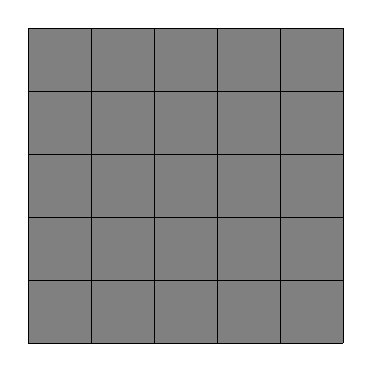
\begin{tikzpicture}[scale=0.8]
        \foreach \x in {0,...,4} {
            \foreach \y in {0,...,4} {
                \fill[gray] (\x,\y) rectangle ++(1,1);
            }
        }
        \draw[step=1cm,ultra thin,black] (0,0) grid (5,5);
    \end{tikzpicture}
    \caption{\centering Cała plansza stanowi ściany.}
    \label{fig:prim_step_1}
\end{figure}

    \item Następnie wybierane jest losowe pole, które zostaje oznaczone jako przejście. Rysunek \ref{fig:prim_step_2} przedstawia wybrane losowo pole startowe.
    
    \begin{figure}[H]
    \centering
    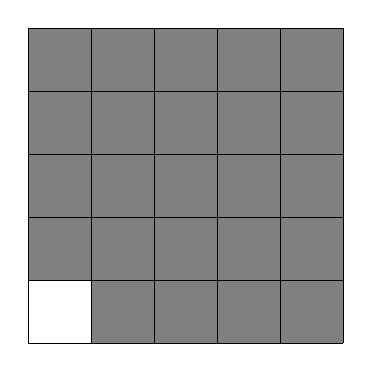
\begin{tikzpicture}[scale=0.8]
        \foreach \x in {0,...,4} {
            \foreach \y in {0,...,4} {
                \fill[gray] (\x,\y) rectangle ++(1,1);
            }
        }
        \fill[white] (0, 0) rectangle ++(1,1);
        \draw[step=1cm,ultra thin,black] (0,0) grid (5,5);
    \end{tikzpicture}
    \caption{\centering Losowe pole startowe.}
    \label{fig:prim_step_2}
\end{figure}

    \item Do zbioru krawędzi dodawane są sąsiednie komórki, do których można przejść bezpośrednio z pola startowego. Za sąsiednie uznaje się komórki oddalone o jedno pole w pionie lub poziomie. Ilustrację tego etapu przedstawiono na rysunku \ref{fig:prim_step_3}.
    
    \begin{figure}[H]
    \centering
    \begin{tikzpicture}[scale=0.8]
        \foreach \x in {0,...,4} {
            \foreach \y in {0,...,4} {
                \fill[gray] (\x,\y) rectangle ++(1,1);
            }
        }

        \fill[white] (0,2) rectangle ++(1,1);
        \fill[pattern=north east lines, pattern color=black] (0,2) rectangle ++(1,1);

        \fill[white] (2,0) rectangle ++(1,1);
        \fill[pattern=north east lines, pattern color=black] (2,0) rectangle ++(1,1);

        \fill[white] (0, 0) rectangle ++(1,1);

        \draw[step=1cm,ultra thin,black] (0,0) grid (5,5);
    \end{tikzpicture}
    \caption{\centering  Wybór sąsiednich pól.}
    \label{fig:prim_step_3}
\end{figure}

    \item Losowana jest jedna krawędź ze zbioru potencjalnych przejść. Jeśli prowadzi ona do nieodwiedzonego pola, tworzy się przejście między bieżącym polem a nowym (usuwana jest ściana między nimi), a nowe pole zostaje oznaczone jako przejście. Następnie do zbioru krawędzi dodawani są sąsiedzi nowo odwiedzonego pola. Ilustrację tego etapu przedstawiono na rysunku \ref{fig:prim_step_4}.

    \begin{figure}[ht]
    \centering
    \begin{tikzpicture}[scale=0.8]
        \foreach \x in {0,...,4} {
            \foreach \y in {0,...,4} {
                \fill[gray] (\x,\y) rectangle ++(1,1);
            }
        }

        \fill[white] (0,2) rectangle ++(1,1);
        \fill[pattern=north east lines, pattern color=black] (0,2) rectangle ++(1,1);

        \fill[white] (2,2) rectangle ++(1,1);
        \fill[pattern=north east lines, pattern color=black] (2,2) rectangle ++(1,1);

        \fill[white] (4,0) rectangle ++(1,1);
        \fill[pattern=north east lines, pattern color=black] (4,0) rectangle ++(1,1);


        \fill[white] (0, 0) rectangle ++(1,1);
        \fill[white] (2, 0) rectangle ++(1,1);
        \fill[white] (1, 0) rectangle ++(1,1);
        \draw[->, very thick, black] (0.5,0.5) -- (2.5,0.5);

        \draw[step=1cm,ultra thin,black] (0,0) grid (5,5);
    \end{tikzpicture}
    \caption{\centering Utworzenie krawędzi do sąsiedniego pola.}
    \label{fig:prim_step_4}
\end{figure}

    \item Proces powtarza się, aż zbiór krawędzi stanie się pusty, co oznacza, że wszystkie komórki zostały połączone.

    Na rysunku \ref{fig:prim_later_steps_a} przedstawiono wyznaczanie kolejnych krawędzi labiryntu, a na rysunku \ref{fig:prim_later_steps_b} końcowy labirynt powstały na podstawie tych krawędzi.
    
    \begin{figure}[ht]
    \centering
    \begin{subfigure}{0.45\textwidth}
        \centering
        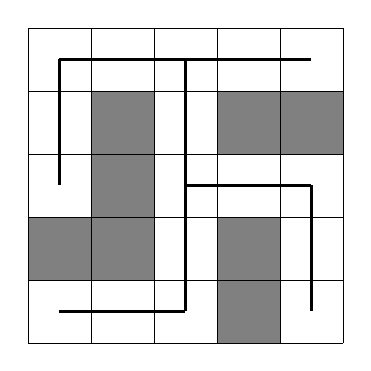
\begin{tikzpicture}[scale=0.8, every node/.style={circle,draw,minimum size=8mm}]
            \draw[very thick, black] (0.5,0.5) -- (2.5,0.5);
            \draw[very thick, black] (2.5,0.5) -- (2.5,4.5);
            \draw[very thick, black] (0.5,4.5) -- (4.5,4.5);
            \draw[very thick, black] (0.5,4.5) -- (0.5,2.5);
            \draw[very thick, black] (4.5,2.5) -- (4.5,0.5);
            \draw[very thick, black] (2.5,2.5) -- (4.5,2.5);

            \fill[gray] (0, 1) rectangle ++(1,1);
            \fill[gray] (1, 1) rectangle ++(1,1);
            \fill[gray] (1, 2) rectangle ++(1,1);
            \fill[gray] (1, 3) rectangle ++(1,1);
            \fill[gray] (3, 3) rectangle ++(1,1);
            \fill[gray] (4, 3) rectangle ++(1,1);
            \fill[gray] (3, 0) rectangle ++(1,1);
            \fill[gray] (3, 1) rectangle ++(1,1);

            \draw[step=1cm,ultra thin,black] (0,0) grid (5,5);
        \end{tikzpicture}
        \caption{\centering Wyznaczanie kolejnych krawędzi labiryntu.}
        \label{fig:prim_later_steps_a}
    \end{subfigure}
    \begin{subfigure}{0.45\textwidth}
        \centering
        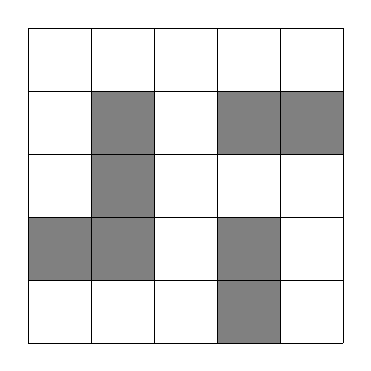
\begin{tikzpicture}[scale=0.8, every node/.style={circle,draw,minimum size=8mm}]
            \fill[gray] (0, 1) rectangle ++(1,1);
            \fill[gray] (1, 1) rectangle ++(1,1);
            \fill[gray] (1, 2) rectangle ++(1,1);
            \fill[gray] (1, 3) rectangle ++(1,1);
            \fill[gray] (3, 3) rectangle ++(1,1);
            \fill[gray] (4, 3) rectangle ++(1,1);
            \fill[gray] (3, 0) rectangle ++(1,1);
            \fill[gray] (3, 1) rectangle ++(1,1);

            \draw[step=1cm,ultra thin,black] (0,0) grid (5,5);
        \end{tikzpicture}
        \caption{\centering Labirynt powstały na podstawie wyznaczonych krawędzi.}
        \label{fig:prim_later_steps_b}
    \end{subfigure}
    \caption{Kolejne kroki działania algorytmu.}
    \label{fig:prim_later_steps}
\end{figure}
\end{enumerate}